\section{Machine Learning Theory}
% Husk reference til Deep Learning bog. Introduction
ML is a branch of AI, where the AI systems must acquire their own knowledge, which they do by extracting patterns from raw data. Some of the tasks that ML can help solve are classification, regression, transcription, and machine translation. DL is a specific kind of ML. It is easy for AI in general to solve problems that can be described by some well-defined mathematical rules. However, initially, AI struggled to do well on tasks that were easy for humans to perform. An example is object recognition in images. While a human, in most cases, can easily distinguish between dogs and cats, the problem is not so easy to translate into mathematical rules that a computer can understand. DL uses NNs, which often consist of many layers, which give rise to the name 'deep' learning \citep{goodfellow2016}. In this thesis, I will focus on solving the classification problem by training a NN in an untraditional way compared to standard NN training. 

% Husk reference til Deep Learning bog. Chapter 6. 
\subsection{Feedforward Neural Networks}
Feedforward NNs are also called multilayer perceptrons (MLPs) and they are one of the simplest NNs. In terms of the classification problem, the goal of a feedforward network is to map an input $\mathbf{x}$ to a class $y$. As such, a MLP defines a mapping $\mathbf{y} = f(\mathbf{x}; \boldsymbol{\theta})$. The goal is then to learn the parameters $\boldsymbol{\theta}$ such that it gives the best function approximation. A MLP is represented by composing together different functions. Two functions, $f^{(1)}$ and $f^{(2)}$ can be used to form $f(\mathbf{x}) = f^{(2)}(f^{(1)}(\mathbf{x}))$. The input is $\mathbf{x}$, $f^{(1)}$ is called the first layer of the network, and $f^{(2)}$ is the second layer, which in this case is also the last layer of the network, called the output layer. During training, each example $\mathbf{x}$ comes with a label $y \approx f^*(\mathbf{x})$ and the goal of the output layer is to produce values, for each $\mathbf{x}$ that is close to the corresponding $y$. The behavior of the remaining layers is not specified. During training, the network must decide how to use those layers, called hidden layers, to produce the desired output. An example of a feedforward neural network is given in Figure \ref{nn}. Given an input vector $\mathbf{x}$, the preactivation $s_{v}^l(\mathbf{x})$ of neuron $v$ in layer $l$ and its activation or output by $a_{v}^l(\mathbf{x})$ can be represented by:

\begin{align*}
    s_{v}(^l \mathbf{x}) = \sum _{u \in N_{l-1}} w_{uv}^l \cdot a_{u}^{l-1}(\mathbf{x})
    \quad 
    \text{and}
    \quad 
    a_{v}^l(\mathbf{x}) = p(s_{v}^l(\mathbf{x}))
\end{align*}
where $N_{l-1}$ is the set of neurons at layer $l-1$ and $p$ is an activation function, which is often an nonlinear function. The default recommendation is to use the rectificied linear unit (ReLU), which is defined as $g(z) = \max(0, z)$, but many other activation functions are possible. The activation function is only applied in the hidden layers. In the input layer, the output is simply equal to the input, and in the output layer, the preactivation values fed into a loss function, that then may send them through a different activation function. 
\begin{figure}[H]
    \centering
    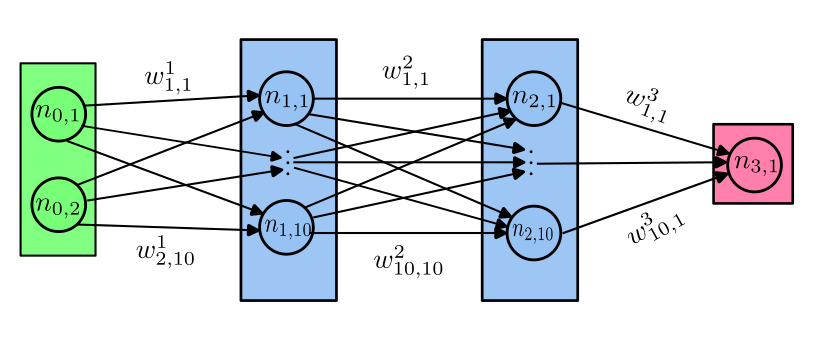
\includegraphics[width=1\linewidth]{Figures/neural_network.png}
    \caption{\small{\textbf{A feedforward neural network with 2 inputs, 2 hidden layers with 10 neurons each, and 1 output neuron. I use the notation $n_{lv}$ to represent neuron $v$ from layer $l$ and $w^l_{uv}$ to represent the weight from neuron $u$ in layer $l-1$ to the neuron $v$ in layer $l$.}}}
    \label{nn}
\end{figure}

\subsection{The Classification Problem}
Classification is a supervised machine learning method, in which training samples have class labels, and the goal is to find a model such that the model performs well on new unseen test samples. In this thesis, I will work with binary classification, in which the model needs only to distinguish between two class labels, and multi-class classification, where the number of class labels is greater than two. The most commonly used loss function, or in LS terminology, objective function used to train NNs, is the cross-entropy function, defined as:

\begin{align}
    \label{cross-entropy} H(P,Q) = -\mathbb{E}_{X \sim P} \log Q(x)
\end{align}
Intuitively, the cross-entropy measures the distance between two probability distributions, and in ML this is often used in gradient descent algorithms to minimize the loss. In this context, $P$ is the true probability distribution, and $Q$ is the predicted. \\ 

\noindent Cross-entropy comes from information theory, but the cross-entropy quantity is actually also closely related to maximum likelihood estimation (MLE) \citep{goodfellow2016}. If we denote the actual distribution of the training data by $p_{\text{data}}(\mathbf{x})$ and let $p_{\text{model}}(\mathbf{x}; \boldsymbol{\theta})$ be the probability distribution that tries to describe the actual distribution of the training data, then the goal is to find $\boldsymbol{\theta}$, so that $p_{\text{model}}(\mathbf{x}; \boldsymbol{\theta})$ is as high as possible. Assuming that there are $m$ examples, $X = \{ x^{(1)}, \ldots, x^{(m)} \}$ drawn independently, from the true but unknown data generating distribution $p_{\text{data}}(\mathbf{x})$, the MLE estimator for $\boldsymbol{\theta}$ is defined as: 

\begin{align*}
    \boldsymbol{\theta}_{\text{ML}} &=  \underset{\boldsymbol{\theta}}{\arg \max} \;  p_{\text{model}} (X; \boldsymbol{\theta}) \\
    & = \underset{\boldsymbol{\theta}}{\arg \max} \; \prod_{i=1} ^m p_{\text{model}} (\mathbf{x}^{(i)}; \boldsymbol{\theta})
\end{align*}
where the rewriting is allowed because of the assumption of independence. This is known as the likelihood function. The goal is to maximize it, and by taking the logarithm of it, the $\arg \max$ is not changed, but it transforms the product into a sum:

\begin{align*}
    \boldsymbol{\theta}_{\text{ML}} = \underset{\boldsymbol{\theta}}{\arg \max} \; \sum_{i=1} ^m \log p_{\text{model}} (\mathbf{x}^{(i)}; \boldsymbol{\theta})
\end{align*}
The $\arg \max$ does not change when rescaling, so dividing by $m$, we obtain a version of the estimate that is expressed as an expectation with respect to the empirical distribution, $\hat{p}_{\text{data}}$ defined by the training data:

\begin{align*}
    \boldsymbol{\theta}_{\text{ML}} = \underset{\boldsymbol{\theta}}{\arg \max} \; \mathbb{E}_{X \sim \hat{p}_{\text{data}}} \log p_{\text{model}} (\mathbf{x}; \boldsymbol{\theta})
\end{align*}
Maximizing this is equivalent to minimizing equation (\ref{cross-entropy}), where $p_{\text{model}}(\mathbf{x}; \boldsymbol{\theta})$ is the predicted probabilities, and $\hat{p}_{\text{data}}$ is the true probability distribution. Normally in supervised learning, we are interested in the case of predicting $\mathbf{y}$ given $\mathbf{x}$, so the goal is to estimate the conditional probability $P(\mathbf{y} \mid \mathbf{x}; \boldsymbol{\theta})$. Denoting by $\mathbf{X}$ all the inputs and $\mathbf{Y}$ all the targets, then the conditional MLE estimator is:

\begin{align*}
    \boldsymbol{\theta}_{\text{ML}} &= \underset{\boldsymbol{\theta}}{\arg \max}P(\mathbf{Y} \mid \mathbf{X}; \boldsymbol{\theta}) \\
    & = \underset{\boldsymbol{\theta}}{\arg \max} \; \sum_{i=1} ^m \log P (\mathbf{y} ^{(i)} \mid \mathbf{x}^{(i)}; \boldsymbol{\theta})
\end{align*}





\subsubsection{Binary Classification Example}
For binary classification, only a single neuron is needed in the output layer. Here, the training samples can be labeled by '0' and '1' respectively, and the preactivation value at the neuron in the output layer can then be used to calculate the probability that the training sample is labeled as '1', denoted by $\hat{y}$, and consequently, the probability that it is labeled as '0' is then given by $1 - \hat{y}$\\
\noindent Suppose we are in a setting where we train a binary classifier and we have a training sample labeled '1', $y=1$, and its preactivation value at the output neuron is -2. We want to know what the binary cross-entropy loss is. As a first step, we need to figure out what the probability of $y = 1$ is. To do this, we use the logistic function to get the predicted probability, $\hat{y}$:
\begin{align*}
    \hat{y} = \frac{1}{1 + \exp(-2)} \approx 0.1192 
\end{align*}
To get the loss, we use the formula from (\ref{cross-entropy}):
\begin{align*}
    H(P,Q) = - \sum_i p_i \log q_i = -y \log \hat{y} - (1-y) \log(1-\hat{y}) = - \log{0.1192} \approx 2.1269
\end{align*}
The loss is quite large since the correct label is '1', and the preactivation value is negative. In binary classification, whenever the label is '1', the preactivation value should be as large as possible to get the highest predicted probability. 

\subsubsection{Multi-class Classification}
The example and intuition above generalizes to multi-class classification, however, now the number of neurons in the output layer needs to be equal to the number of classes. In this case, we cannot use the logistic function anymore to get the predicted probability. Instead, we take the vector of preactivation values from the output layer and apply the softmax function to it, which gives a vector of probabilities for each class such that the probabilities sum up to 1. Formally, given the vector $z$ with preactivation values, this is defined as: 

\begin{align}
    \label{softmax} \text{softmax} (\mathbf{z})_j = \frac{\exp(z_j)}{\sum_{k=1}^m \exp(z_k)}
\end{align}
where $m$ is the number of classes and the classes are labeled $1, \ldots, m$. The cross-entropy loss, is, however, easier to calculate in this case using (\ref{cross-entropy}), as this reduces to the negative of the logarithm of the probability for the right label:
\begin{align*}
    H(P,Q) = - \log \frac{\exp(z_y)} {\sum_{k=1}^m \exp(z_k)}
\end{align*}



\subsection{Traditional Neural Network Training}
Optimization algorithms within ML and DL differ from traditional optimization problems. In ML, it is the goal to perform well on some unknown test set, which is in contrast to traditional optimization problems, where solving the problem at hand is the task. To measure the performance of a ML model, the model is tested on a held-out test set. This is used to estimate how well the model generalizes. It can be beneficial to divide the remaining training set into two disjoint sets - a final training set and a validation set. The validation set can be used during training for model selection or hyperparameter selection, but it is not used to train the main parameters of the model. The test set is not seen until after the entire training process, and as such, it is only seen once, while the validation set can be seen many times. \\ 

\noindent For classification, we are concerned about predicting as many samples in the test set correctly as possible. To evaluate a classification model, a well-known performance measure is the 0-1 loss, which basically returns the error rate, however, this loss-function is not well-suited for optimization tasks, neither in traditional NN training nor in a LS context. In traditional NN training, a surrogate loss function is used instead, which could be the cross-entropy loss function introduced earlier. Some reasons for this are that the 0-1 loss is non-differentiable, non-continuous, and it does not give as robust a model as when using the cross-entropy loss function. To prevent overfitting, which occurs when the training error is small, but the test error is large, it is possible to use an early stopping technique, where the model trained is tested at certain times on the validation set. Here, it is often the 0-1 loss that is used and the model with the smallest loss is then chosen, even though a later model might have a smaller loss when using the surrogate function. \\ 

\noindent The most common optimization algorithm within ML and especially DL is stochastic gradient descent (SGD). SGD works by sampling a small subset of samples from the training set. Sometimes this is referred to as a minibatch, but herein I will use the term 'batch'. The batch is then used to compute the gradients of the parameters, and very small updates are made to the parameters. In Algorithm \ref{sgd}, the pseudocode of a simple version of SGD can be seen. In practice, the convergence criterion is often replaced by iterating over the entire training set for a certain number of epochs, and the learning rate, which is a very sensitive hyperparameter, should decrease during the training. Many extensions of this, conceptually simple, algorithm exist. Some of these extensions try to overcome some of the challenges that arise when training NNs. To accelerate learning, momentum can be introduced, or to overcome the problem of choosing the correct learning rate, algorithms with adaptive learning rates can be used, which however, introduce more hyperparameters. Early stopping can be applied by testing the model on the validation set after each time the entire training set has been seen, called an epoch. 

\begin{algorithm}
\caption{Pseudocode for Stochastic Gradient Descent} \label{sgd}
\begin{algorithmic}
    \State \textbf{Require:} Learning rate $\epsilon$ 
    \State \textbf{Require:} Initial parameter $\boldsymbol{\theta}$
    \While {Convergence criterion is not met}
        \State Sample a batch from the training set 
        \State Compute gradient estimate $\boldsymbol{\hat{g}}$
        \State Apply update: $\boldsymbol{\theta} \leftarrow \boldsymbol{\theta -} \epsilon \boldsymbol{\hat{g}}$
    \EndWhile
\end{algorithmic}
\end{algorithm}

\subsection{Binary Neural Networks}
% Evt. kilde til Hubara. 
The development in the use of NNs has pushed the limits of AI significantly, however, before the introduction of BNNs, the NNs were trained using one or many GPUs. This means that it is a challenge to run NNs on low-power devices. BNNs are networks, where weights and activations are limited to be either -1 or 1. \cite{Hubara2016} showed that it was possible to train BNNs without suffering any loss in classification accuracy. They used the traditional gradient descent approach and then made several tricks to come up with a solution that handles the challenges of training BNNs in this way. Normally, the gradient update in Algorithm \ref{sgd} is based on the gradients found by backpropagation, but for BNNs the gradient of the sign function used to binarize the weights is zero almost everywhere. Instead, they use an estimator for this gradient called the straight through-estimator. With their training approach, they compute the real-valued gradients during the backward pass, and only binarize during the forward pass. How to train BNNs using traditional GD methods has been an active research area and it is beyond the scope of this thesis to give a full overview. For a more comprehensive review, I refer to \cite{yuan2023}. 

\subsection{Ensemble Methods}
In ML, ensemble methods are powerful techniques that combine the predictions of multiple models to improve overall performance and robustness. Two of the most well-known ensemble methods are bagging and boosting. \\

\noindent Bagging, short for Bootstrap Aggregating, involves creating $k$ different datasets. Each dataset is constructed by randomly sampling from the original dataset with replacement. This process generates $k$ datasets, each containing duplicates of some examples while others are omitted. $k$ models are then trained on these different datasets, and their predictions are aggregated through voting, leading to a more stable and accurate final prediction. \\

\noindent Boosting, on the other hand, trains several models sequentially on the same dataset. The key idea is to assign weights to the training examples, adjusting them after each model is trained. If a model $i$ misclassifies certain examples, these examples are given higher weights for the training of model $i+1$. This ensures that the new model focuses more on the difficult cases, improving the overall performance. \\

\noindent In this thesis, I implement the BeMi ensemble introduced by \cite{ambrogio2023}. Given a set of classes $C$ in a classification problem, this ensemble trains $\binom{\vert C \vert} {2}$ different neural networks, each designed to distinguish between two distinct classes from $C$. The idea is to pass the inputs through all these networks. If all networks trained on the true label of the input classify it correctly, then at most $\binom{\vert C \vert - 1}{2-1} - \binom{\vert C \vert - 2}{2-2}$ other networks can misclassify the input, ensuring the ensemble's correct classification. \\

\noindent MNIST is a widely recognized dataset used for classifying handwritten digits ranging from 0 to 9. For this task, $\binom{10}{2} = 45$ binary classifiers are required, each trained to differentiate between pairs of digits. When a test example is classified, it is fed into all 45 networks. If all 9 networks that have encountered the test example's true label classify it correctly, then at most $\binom{9}{1} - \binom{8}{0} = 8 $ other networks can misclassify it, ensuring the correct prediction. A test example can also be classified correctly when two labels receive the same number of votes. In this case, the network trained to distinguish between these two labels is used to break the tie. If this network's prediction is correct, it also counts as a correct prediction.
